%% LyX 2.1.1 created this file.  For more info, see http://www.lyx.org/.
%% Do not edit unless you really know what you are doing.
\documentclass[twoside,english]{article}
\usepackage[utf8]{luainputenc}
\usepackage[a4paper]{geometry}
\geometry{verbose,tmargin=3.5cm,bmargin=3cm,lmargin=3cm,rmargin=3cm}
\setlength{\parskip}{\medskipamount}
\setlength{\parindent}{0pt}
\usepackage{array}
\usepackage{float}
\usepackage{url}
\usepackage{graphicx}

\makeatletter

%%%%%%%%%%%%%%%%%%%%%%%%%%%%%% LyX specific LaTeX commands.
\providecommand{\LyX}{L\kern-.1667em\lower.25em\hbox{Y}\kern-.125emX\@}
%% Because html converters don't know tabularnewline
\providecommand{\tabularnewline}{\\}

%%%%%%%%%%%%%%%%%%%%%%%%%%%%%% Textclass specific LaTeX commands.
\newenvironment{lyxlist}[1]
{\begin{list}{}
{\settowidth{\labelwidth}{#1}
 \setlength{\leftmargin}{\labelwidth}
 \addtolength{\leftmargin}{\labelsep}
 \renewcommand{\makelabel}[1]{##1\hfil}}}
{\end{list}}

%%%%%%%%%%%%%%%%%%%%%%%%%%%%%% User specified LaTeX commands.
\usepackage{fancyhdr}
\usepackage{afterpage}
\usepackage{framed}
\usepackage{settings}
\usepackage{lscape}
\usepackage{pdflscape}
\usepackage{color}   %May be necessary if you want to color links
\usepackage{hyperref}

%Set up settings
\setcounter{secnumdepth}{4}
\usepackage{hyperref}
\hypersetup{
    linktoc=all,     %set to all if you want both sections and subsections linked
}

\makeatother

\usepackage{babel}
\usepackage{listings}
\renewcommand{\lstlistingname}{Listing}

\begin{document}
\pagestyle{empty}

\begin{titlepage}

\begin{center}
\Large{\textsc{Politecnico di Milano}}\\
\Large{Scuola di Ingegneria Industriale e dell'Informazione}\\
\large{M.Sc. in Computer Science and Engineering}\\
\large{Dipartimento di Elettronica, Informazione e Bioingegneria}
\par\end{center}

\vspace{0.3cm}


\begin{center}
\begin{figure}[h]
\centering{}
\includegraphics[width=0.4\textwidth]{title-page/logo}
\end{figure}
\vspace{0.4cm}

\par\end{center}

\begin{center}
\huge{\textbf{myTaxiService}}\\
\vspace{0.2cm}

\par\end{center}

\begin{center}
\Large{Software Engineering 2 - Project}
\par\end{center}

\begin{center}
\vspace{0.9cm}
\Huge{\textbf{RASD}}\\
\Large{\textbf{Requirements Analysis and }\\
\textbf{Specification Document}}
\par\end{center}

\begin{center}
version 1.0
\par\end{center}

\begin{center}
6th November 2015
\par\end{center}

\begin{flushleft}
\vspace{0.5cm}

\par\end{flushleft}

\begin{flushright}
\begin{tabular}{ll}
Authors: & \tabularnewline
Alberto Maria METELLI & Matr. 850141\tabularnewline
Riccardo MOLOGNI & Matr. 852416\tabularnewline
\end{tabular}
\par\end{flushright}

\begin{flushleft}
\vspace{1.8cm}

\par\end{flushleft}

\begin{center}
{\large{}Academic Year 2015–2016}
\par\end{center}{\large \par}

\end{titlepage}


\clearpage{}

\afterpage{\null\newpage}

\clearpage{}

\pagestyle{fancy}
\fancypagestyle{plain}
\fancyhf{}
\fancyfoot{}
\fancyhead[LE,RO]{\thepage} 
\fancyhead[LO]{\slshape \rightmark} 
\fancyhead[RE]{\slshape \leftmark} 

\thispagestyle{empty}
\pagenumbering{roman}\tableofcontents{}\listoffigures


\clearpage{}

\pagenumbering{arabic}

\thispagestyle{empty}


\section{Introduction}


\subsection{Purpose}

The purpose of the RASD \emph{(Requirements Analysis and Specification
Document}) is to give a detailed description, analysis and specification
of the requirements for the \emph{myTaxiService} software. This document
will explain the \emph{goals} coming from stakeholders' expectations,
the characteristics of the application domain and the \emph{assumptions}
made to solve ambiguity and incompleteness. Starting from goals and
domain properties, \emph{requirements} will be formulated according
to a specific systematic methodology and then specified using both
informal and formal notations. However this document should not be
considered the final draft for the software specifications since in
the following phases several fixing may be necessary. 

The main objective of the RASD is to achieve good understanding among
\emph{analysts, developers, testers} and \emph{customers}, in particular
explaining both the application domain and the system to-be; it is
also aimed to be a solid base for project planning, software evaluation
and possible future maintenance activities. Therefore this document
is primarily intended to be proposed to the stakeholders for their
approval, to the analysts and programmers for the development of the
project and to the testing team the validation of the first version
of the software.


\subsection{Present system}

At the moment taxi service is entirely managed by phone calls. A passenger
who wants to request or reserve a taxi has to contact the call center.
In case of request, the call center operator moves the call to the
first available taxi, otherwise, in case of reservation, a taxi is
booked for the specific date, time and address provided by the passenger.
No available taxi queues management is implemented at the moment. 


\subsection{Scope}

The \emph{myTaxyService} is an application intended to optimize taxi
service in a large city, making the access to service simpler for
the passengers and ensuring a fair management of the taxi queues. 

Passengers will be able to request a taxi either through a web application
or a mobile app; of course the ``traditional'' ways to call for
a taxi, like a phone call or stopping the taxi along the road, will
be still available and integrated into the system to-be. The software
will make the procedure of calling a taxi simpler (by using GPS information
passenger doesn't need to know the address if the taxi is needed for
the current position) and more usable (passenger will be provided
with information about the waiting time). Moreover, by means of the
application, the passenger can reserve a taxi for a certain date and
time, specifying the origin and the destination of the ride.

Taxi drivers will use a mobile app to inform the system about their
availability and to confirm that they are going to take care of a
call (or to reject it for any reason). The software will make the
taxi management more efficient: the system will be able to identify
the position of each taxi by using GPS; the city will be divided in
virtual zones and a suitable distribution of the taxi among the zones
will automatically be computed.


\subsection{Definitions, acronyms, abbreviations }

In this paragraph all the terms, acronyms and abbreviations used in
the following sections are listed.


\subsubsection{Definitions}
\begin{itemize}
\item \emph{Request}: the action performed by the passenger of calling a
taxi for the current position.
\item \emph{Confirmed request}: a request that has been accepted by a taxi
driver.
\item \emph{Reservation}: the action performed by the passenger of booking
a taxi for a specific address and specific date and time.
\item \emph{Waiting time}: an estimation of the time required to taxi driver
to get to passenger's position.
\item \emph{Taxi code}: a unique alphanumerical identifier of the taxi.
\item \emph{Available taxi queues}: data structures used to store the references
of the available taxis, also used to select the taxis to which forward
a request.
\item \emph{Automatic geolocalization}: a system that provides the geographic
coordinates of the user. For this document it can be either a GPS
system or browser geolocalization.
\item \emph{Passengers' application}: the applications used by passengers
to access to TS system. For this document it can be either PMA or
PWA (see 1.4.2).
\item \emph{Login credentials}: username and password.
\item \textit{Notification}: communication from TS to taxi driver to move
to a specific zone.
\end{itemize}

\subsubsection{Acronyms}
\begin{itemize}
\item TS: myTaxiService.
\item PMA: Passenger mobile application.
\item PWA: Passenger web application.
\item TMA: Taxi driver mobile application.
\item QMS: Queue management system.
\end{itemize}

\subsubsection{Abbreviations}
\begin{itemize}
\item {[}Gn{]} n-th goal.
\item {[}Dn{]} n-th domain assumption.
\item {[}Rn.m{]} m-th requirement related to goal {[}Gn{]}.
\end{itemize}

\subsection{Actors}

In this paragraph a brief description of the various actors affected
by myTaxiService system is provided.
\begin{itemize}
\item \emph{Passenger}: a person that interacts with myTaxiService to request
or reserve a taxi. The interaction with the system may occur by means
of either PMA (mobile passenger) or PWA (web passenger). Each passenger
can be either a registered passenger or an unregistered passenger.
\item \emph{Registered passenger}: specific case of passenger that has already
registered to the system. He/She can login, request, reserve a taxi
and also visualize and modify the previous reservations.
\item \emph{Unregistered passenger}: specific case of passenger that hasn't
registered to the system. He/She can only request a taxi.
\item \emph{Taxi driver}: a person that drives a taxi and is associated
with myTaxiService. He/She interacts with the system confirming or
rejecting requests and informing the system about his/her availability
by means of TMA.
\item \emph{Call center operator}: a person working at the call center that
interacts with the system inserting taxi requests coming from phone
calls. 
\end{itemize}

\subsection{Requirement engineering approach}

In order to ensure a sound and complete requirement engineering activity,
we decided to follow a systematic technique for requirements formulation
proposed by Jackson and Zave. This approach is based on the distinction
between the \emph{machine}, the portion of the system to be developed
(myTaxiService in our case), and the \emph{world}, the portion of
the real world interacting with the machine. Machine and world are
tipically non disjoint, some phenomena may affect both of them, they
are known as shared phenomena. From this viewpoint, requirement engineering
consists in identifying phenomena shared between world and machine,
according to a set of \textbf{goals }(which express the desired behavior
of world phenomena, shared or not) and a set of \textbf{domain assumptions}
(assertions supposed to be always valid in the world). Formally a
set of \textbf{requirements }is complete if together with domain assumption
it ensures the goals.


\subsubsection{Goals}

Starting from the available documentation, integrated with some interviews
with the stakeholders, the following minimal goals has been identified.
\begin{lyxlist}{00.00.0000}
\item [{{[}G1{]}}] Allow a passenger to request a taxi for its current
position without registration.
\item [{{[}G2{]}}] Allow the passenger to visualize the waiting time and
the code of the incoming taxi for confirmed requests.
\item [{{[}G3{]}}] Allow a registered passenger to have a personal area.
\item [{{[}G4{]}}] Allow a registered passenger to reserve a taxi.
\item [{{[}G5{]}}] Allow a registered passenger to cancel or modify a previous
reservation. 
\item [{{[}G6{]}}] Allow a taxi driver to either accept or reject a request
coming from the system.
\item [{{[}G7{]}}] Allow a taxi driver to inform the system about his/her
availability.
\item [{{[}G8{]}}] Ensure that available taxi queues enjoy the properties
specified in sub paragraph 1.6.2.
\end{lyxlist}

\subsubsection{Queue management}

This paragraph is aimed to give a more precise definition of ``fair
management'' of the available taxi queues.

The city is divided into several zones, to each zone a taxi queue
is assigned. Each zone is characterized by a different load of requests
$n_{i}$ measured in request/minute. Let $N$ be the total number
of taxis available at a certain moment, the number $q_{i}$ of taxis
available in the zone $i$ has to be proportional to $n_{i}$, in
particular $q_{i}=Nn_{i}/\sum_{i}n_{i}$. Every time one taxi turns
from available to busy or out of service or viceversa a new distribution
of the taxis has to be computed; the taxis to be moved have to minimize
the cost of movement calculated as number of zones passed through.
To prevent too many movements, a fluctuation between -30\% and 30\%
from the value $q_{i}$ is accepted without performing taxi movements.


\subsection{Reference documents }
\begin{lyxlist}{00.00.0000}
\item [{{[}1{]}}] IEEE Software Engineering Standards Committee, “IEEE
Std 830-1998, IEEE Recommended Practice for Software Requirements
Specifications”, October 20, 1998. 
\item [{{[}2{]}}] P, Zave, M. Jackson, Four dark corners of requirements
engineering, TOSEM 1997.
\item [{{[}3{]}}] Software Abstractions: Logic, Language, and Analysis,
revised edition Edition by Daniel Jackson, MIT Press.
\item [{{[}4{]}}] Software Engineering 2 course slides.
\end{lyxlist}

\subsection{Overview}

This document is drawn up in accordance to the IEEE Std 830-1998 for
Software Requirements Specifications and it is composed of four sections
and an appendix.
\begin{itemize}
\item The first, this one, section gives a general description of the document
and brief information about the actors and the purposes of the software.
\item The second section provides an overview of the software, highlighting
the interaction with external system interfaces and explaining the
main functions carried out. It also focuses on constraints and domain
assumptions.
\item The third section is entirely dedicated to the derivation and specification
of the requirements. Several scenarios expressed in natural language
will be provided. A generalization of the set of scenarios will be
specified as a set of use cases that will be expressed both in natural
language and using UML use case diagram. For some groups of use cases
a dynamical description will be provided mainly using UML sequence
diagram. A high level conceptual description of the classes affected
by the system will be given using UML class diagram. For some of the
objects involved, we will design a UML state chart diagram showing
the evolution of its state. 
\item The fourth section presents a formalization of a subset of the requirements
using Alloy; some significant instances will be shown.
\item The appendix contains an interesting model of the goals, a brief description
of the tools used to produce this documents and the number of hours
each group member has worked towards the fulfillment of this deadline.\end{itemize}



\clearpage{}

\thispagestyle{empty}


\section{Overall description}


\subsection{Product perspective }

\emph{myTaxiService} (TS) software can be decomposed into four different
interacting subsystems (Figure 1):
\begin{enumerate}
\item the \emph{passenger web application} (PWA): it's a web portal that
allows passenger to request a taxi, register, login, reserve a taxi
and cancel or modify previous reservations. PWA has to be able to
identify passenger's position using, if available, the browser geolocalization
support.
\item the \emph{passenger mobile application }(PMA): it's an application
that shall be installed on passengers' smartphone performing the same
functions of PWA. PMA needs also to communicate to a GPS application
within the mobile phone, if any available, to retrieve the passenger's
position.
\item the \emph{taxi driver mobile application} (TMA): it's an application
that shall be installed on taxi drivers' smartphone in order to allow
them to receive requests coming from the system, decide to confirm
or reject requests and inform the system about their availability. 
\item the \emph{queue management system} (QMS): it's a software aimed to
compute realtime the distribution of the taxis in the city interfacing
with the GPS system of each taxi, decide which taxi assign to a request
and send to taxi drivers several notifications.
\end{enumerate}
TS has also to be integrated with the previous taxi management system
based on phone calls in order to allow call center operators to forward
requests, therefore a specific interface shall be designed. Moreover,
the system has to be provided with specific interfaces and APIs in
order to allow future requirements extensions.

\begin{figure}
\begin{centering}
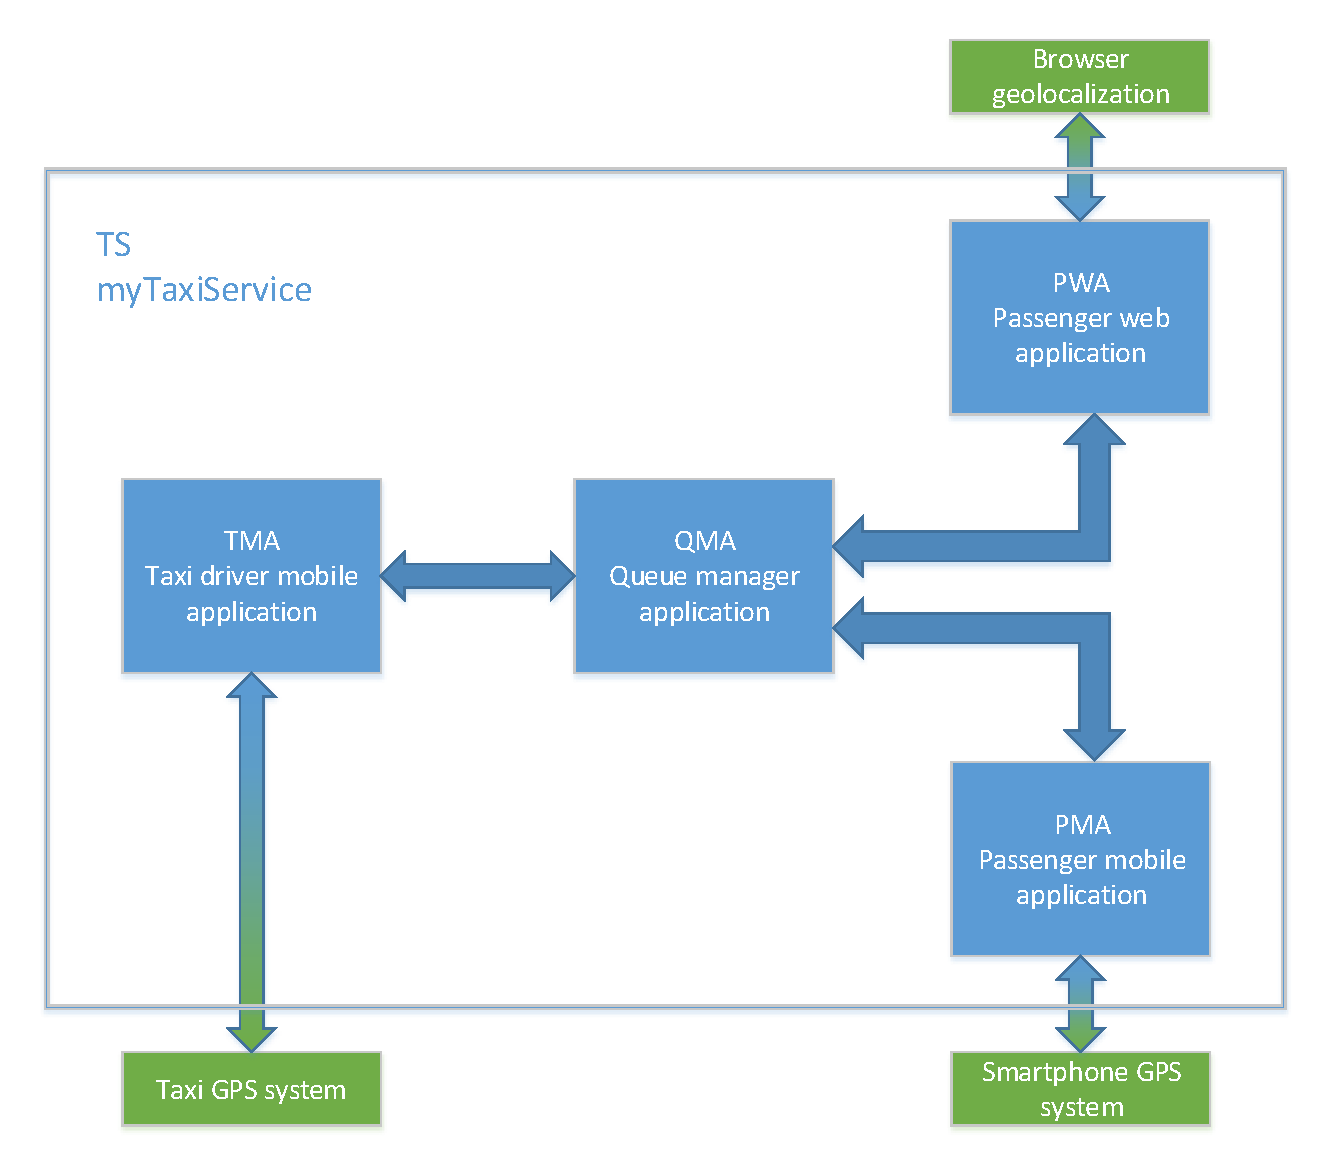
\includegraphics[scale=0.5]{overall-description/Diagram}
\par\end{centering}

\protect\caption{Block schema representing the conceptual interaction between subsystems.}


\end{figure}



\subsection{User characteristics}

Main addressee of myTaxiService are passengers and taxi drivers. Users
are not expected to have specific knowledge or technical expertise
but it is assumed they are able to operate the internet and to have
access to it.


\subsection{Constraints }


\subsubsection{Regulatory policies}

The following regulatory policies has to be met by the software.
\begin{itemize}
\item Since user's geographic position needs to be shared within the application
(either PMA or PWA) to ensure the expected behavior of the system,
users has to agree in advance to specific terms and conditions. 
\item Taxi drivers are obliged not to spread possible collected information
about passengers.
\end{itemize}

\subsubsection{Hardware limitations }

The following hardware limitations has to be met.
\begin{itemize}
\item Mobile passengers has to download the free application from the store
(PlayStore for Android users, AppStore for iPhone users, Windows store
for Windows users). It is assumed that the mobile phones have enough
primary memory to run the application.
\item The browser used by web passengers to access the system must have
cookies enabled.
\item Each taxi driver is provided with a smartphone and the application
TMA must be installed.
\end{itemize}

\subsection{Domain assumptions}

Considering the specific application domain and according to the information
provided by stakeholders we can assume that the following assertions
are always valid.
\begin{lyxlist}{00.00.0000}
\item [{{[}D1{]}}] A taxi driver always executes indications communicated
by the system (e.g. move notifications), except in case of emergency.
\item [{{[}D2{]}}] Each taxi is provided with a GPS system. If GPS system
is not available taxi is considered out of service.
\item [{{[}D3{]}}] A taxi can be stopped along the road by a passenger
if and only if it is waiting without passenger or moving but not for
carrying out a request. In this case taxi driver informs the system
about his/her unavailability.
\item [{{[}D4{]}}] When a taxi driver finishes to carry out a request he/she
informs the system about his availability.
\item [{{[}D5{]}}] When a taxi driver starts his work-shift sets his/her
state from out of service to available.
\item [{{[}D6{]}}] When a taxi driver ends his work-shift if the current
state is available then the taxi state becomes out of service; otherwise
taxi driver finishes to carry out the current request and after that
the taxi becomes out of service.
\item [{{[}D7{]}}] When a taxi driver gets to the meeting place, waits
for 10 minutes; if passenger does not arrive taxi driver informs the
system.
\item [{{[}D8{]}}] A taxi is assigned to a unique taxi driver at time.
It is possible that some taxi drivers are not assigned to any taxi
or vice versa.
\item [{{[}D9{]}}] If a ride gets out of the city the taxi driver comes
back to the last zone before informing TS of his availability.
\item [{{[}D10{]}}] There are only two types of taxi: normal (4 seats)
and minivan (9 seats).
\item [{{[}D11{]}}] Each available taxi belongs to exactly one queue at
time. Busy or out of service taxis do not belong to any queue.
\item [{{[}D12{]}}] TS is available only in the city, no requests coming
from outside of the city boundary are accepted.
\item [{{[}D13{]}}] Taxi drivers have always access to the Internet.
\item [{{[}D14{]}}] Taxi drivers' work-shifts are managed in order to ensure
that at each moment the number of in service taxis is at least 50\%
of the total number of taxis.
\item [{{[}D15{]}}] Taxi drivers go in emergency state only in case of
car accident or similar events.
\item [{{[}D16{]}}] Taxi can move without limitations inside the zone assigned
by TS system but they cannot change the zone without a notification
from the system.
\end{lyxlist}
Note that also taxi drivers are identified by the system but registration
of the taxi driver is not part of the TS system since it reasonably
involves contractual issues (taxi driver has to make an agreement
with the company) that cannot be directly managed by the system. Therefore
registration is not performed by taxi driver.


\subsection{Possible future extensions}

The following are reasonable possible future extensions to the TS
system; they are mainly meant to further improve the usability and
the performances of the service. They will not be discussed in details.
\begin{itemize}
\item At present, queues has a fixed suitable number of available taxis
which is supposed to be calculated using previous data about the number
of requests coming from each zone. However the distribution of the
requests can vary not only \emph{spatially} (from one zone to an other)
but also \emph{temporally} (for each zone at different moments of
the day the number of requests might be different). Also in different
days of the week the distribution of requests may vary significantly.
A possible solution to make TS more adaptive is the one in which the
suitable number of taxis for each queue is periodically determined
integrating data collected from the requests in a certain time horizon
(for instance once a week).
\item At the moment TS system does not handle payments, since users are
expected to pay the ride cash or with credit card to the taxi driver;
online payments can be implemented within TS system. Both PWA and
PMA should allow registered users to pay the price of the ride using
credit card or paypal; cash payment should be still possible.
\item At the moment, passenger requesting a taxi can only see the estimated
waiting time and the code of the taxi, while visualizing also the
current position of the incoming taxi should be more useful.
\item An evaluation system of the quality of service can be added, allowing
passengers to express an opinion about taxis.\end{itemize}



\clearpage{}

\thispagestyle{empty}


\section{Specific Requirements }


\subsection{External Interface Requirements }

\input{\string"specific-requirements/3.1-external-interface-requirements/external interface requirements.tex\string"}

\clearpage{}


\subsection{Functional Requirements }

\input{\string"specific-requirements/3.2-functional-requirements/functional requirements.tex\string"}

\clearpage{}


\subsection{Scenarios}

In order to clarify the expected functionality of the system, in this
subsection we propose several possible scenarios. In each scenario
we emphasize several specific interactions between the users and the
system, but, in some of them, we do not describe the entire process
carried out interacting with TS to avoid useless repetitions.


\subsubsection{Scenario 1}

Bob is an unregistered passenger of TS. He has decided to visit a
friend that lives in another district. He accesses the TS using the
PWA via browser installed on his PC, he specifies his current address
because his PC can’t provide him with browser geolocalization. After
accepting terms and conditions related to the service he confirms
the request. The TS system processes his request and sends a notification
to Bob. Meanwhile the system sends the request to the first available
taxi in the queue associated to the area where Bob is. The taxi driver,
Tom, after having received the request on his smartphone via TMA,
he confirms it. Tom visualizes the request information details and
leaves from his location to get to the address specified by Bob. TS
system calculates the waiting time and shows it to Bob. When Tom arrives
to Bob's, he picks up him and brings him to his friend. Before leaving
Bob pays Tom for the service and Tom informs the system that he is
available again.


\subsubsection{Scenario 2}

As soon as Alice left the theater it started raining, so she decided
to try TS service for the first time. She uses her 3G connection to
download the PMA and starts it. After that she accepts terms and conditions
of TS, the system retrieves Alice’s current position by means of her
GPS. She confirms the requests and the system contacts the first taxi
available in her zone. Unfortunately it has run out of fuel so, Tim,
the taxi driver is waiting his turn at the gas station and decides
to refuse the request. The system puts the Tim’s taxi at the end of
the queue and sends a request at the second taxi available. Tess,
the new taxi driver, accepts the request, picks up Alice and brings
her to home.


\subsubsection{Scenario 3}

Robb needs to reach the university campus because he has to addend
Software Engineering 2 morning class, so he reaches the bus stop but
he notices a sign informing that an unexpected public transportation
strike is going on. Unfortunately this happens quite often, that's
why Robb is a registered passenger of TS. He logs in the PMA and requests
a taxi. Due to the strike a large number of requests has been forwarded
the system so no taxi is available at the moment in that zone of the
city. Therefore the first taxi in the queue of an adjacent zone is
contacted. The taxi driver, Taylor, accepts the request. The system
shows the expected waiting time on Rob's smartphone. After 15 minutes
Taylor picks up Robb who will get to university, in time for the class.


\subsubsection{Scenario 4}

Arya booked a low cost flight to Marrakesh but the plane leaves early
in the morning so she decided to register on TS website to reserve
a taxi. She filled the registration form with the requested information
and confirmed, accepting terms and conditions. The system sends her
a confirmation e-mail. A few days before the departure she logs in
her personal area on the PWA and reserves a taxi, specifying her address
and the meeting time. The leaving day she hasn't heard the alarm clock
and she hasn't woken up. When Takashi, the taxi driver, arrives at
Arya’s place he doesn’t find anyone so he waits for 10 minutes and
then informs the system. The system puts Takashi's taxi at the end
of the available taxi queue.


\subsubsection{Scenario 5}

In the city a huge sport event has been organized for today so the
city center is closed. Jon wants to reach his house after a stressful
working day. Jon usually comes back home using public transportation
but today it's a mess so he decides to take a taxi. He sends a request
using his PMA but all the taxis in all the zones are busy due to the
unexpected number of people coming to attend the event. The system
informs Jon about the situation and provides Jon with the expected
waiting time: one hour, too much for Jon. So he decides to ask one
of his colleagues for a lift.


\subsubsection{Scenario 6}

Sansa always uses taxis to move in the city because she has never
passed her driving license exam. Today she needs a taxi to reach the
shopping center but unfortunately she doesn't have access to the Internet
so she calls the taxi service phone number. A call center operator,
Trudy, answers the phone and asks the location where the taxi should
pick up her and the number of passengers. Sansa tells him her current
address and says she would be the only passenger. Trudy uses a PWA
to send a request to the TS system and announce to Sansa the expected
waiting time when she receives the confirmation by TS. 


\clearpage{}

\input{\string"specific-requirements/3.4-use-cases/use case.tex\string"}

\clearpage{}

\input{\string"specific-requirements/3.6-other-uml/class diagram and other.tex\string"}

\clearpage{}


\subsection{Non functional requirements}

Since TS system is intended to increase the degree of usability of
the taxi service and perform improvements in the available taxi queue
management, according to stackeholders' expectations we identified
the following non functional requirements.


\subsubsection{Performance}
\begin{itemize}
\item All internal elaborations carried out by QMA must have a response
time of 100 ms in 99\% of times.
\item TMA, PMA and PWA must have a response time of 10 ms in 99\% of times
for local elaborations (not involving Internet connection).
\item Remote interaction (via Internet) within TS system must least at most
2 seconds otherwise the connection is closed.
\item TS system shall support at least 500 simultaneous connections.
\end{itemize}

\subsubsection{Reliability}
\begin{itemize}
\item TS system shall ensure that every operation coming from TMA, PMA and
PWA is correctly processed.
\item All the user inputs are verified by the local application before being
sent to the TS system .
\item TS system shall be a transactional system (both operations generated
by users and internal operations carried out by TS system are transactions).
\end{itemize}

\subsubsection{Availability }
\begin{itemize}
\item The TS system must be available 99.9\%. 
\item A hardware duplicate must be ready to be activated when maintenance
is performed or failure occurs to ensure continuity of the service.
\item A backup of data should be performed every week to prevent any loss
of data in the TS system.
\end{itemize}

\subsubsection{Security }
\begin{itemize}
\item All sensitive data collected from users must be stored in safe devices
accessible only by authorized users to prevent loss, manipulation
or stealing.
\item All data flowing between system and users must be encrypted to ensure
confidentiality.
\item Registered passenger's password must be changed every three months.
\end{itemize}

\subsubsection{Maintainability }
\begin{itemize}
\item TS system shall be developed in order to reduce the maintenance cost,
trying to anticipate and preventing future interventions (corrective
and adaptive maintenance) by means of standard patterns (in particular
the architecture must follow the MVC pattern).
\item TS system shall expose a set of APIs in order to allow future functionalists
extensions (perfective maintenance).
\item Thanks to hardware duplication, hardware maintenance interventions
will be performed without service interruption.
\end{itemize}

\subsubsection{Portability }
\begin{itemize}
\item TMA and PMA shall be installable in both iOS, Android and Windows
mobile.
\item PWA shall be accessible by means of all up to date browsers having
cookies enabled.
\end{itemize}

\subsubsection{Documentation}
\begin{itemize}
\item An accurate user guide must be available online.
\item All the documents produced during the design and development of the
TS shall be available for specialized personnel.
\end{itemize}

\subsubsection{User interface and human factors }
\begin{itemize}
\item TS is meant for user without any particular knowledge or experience
in the field of IT so the application must be intuitive and easy to
master.
\item Every functionality shall be reached surfing no more than 4 pages.\end{itemize}



\clearpage{}

\thispagestyle{empty}


\section{Alloy model}

In this section we provide an alloy model trying to capture the main
features of the entities affected by the TS system. The model is built
defining signatures according to the class diagram and specifying
the constraints that comes out from the requirements.


\subsection{General model}


\subsubsection{Signatures, facts and functions}

\begin{lstlisting}[breaklines=true]
module myTaxiService/model

//Auxiliary signatures 
sig Date{} 
sig Time{}

sig Location{ 	
	zone: one Zone, 
}

abstract sig Passenger{} 
sig UnregisteredPassenger extends Passenger{} 
sig RegisteredPassenger extends Passenger{}

abstract sig TaxiState{} 
one sig OutOfService,Emergency extends TaxiState{} 
one sig Available, Busy, Moving extends TaxiState{}

abstract sig Taxi { 	
	driver: lone TaxiDriver, 	
	state: one TaxiState, 	
	numberOfSeats: one Int, 
}  

sig MinivanTaxi extends Taxi {} {numberOfSeats = 9} 
sig NormalTaxi extends Taxi {} {numberOfSeats = 4}

sig TaxiDriver{}

sig Request{ 	
	passenger: one Passenger, 	
	date: one Date, 	
	time: one Time, 	
	numberOfPassengers: one Int, 	
	location: one Location, 
}  {numberOfPassengers>=1}

sig ConfirmedRequest extends Request{ 	
	waitingTime: one Time, 	
	taxis: some Taxi, 
}

sig Reservation{ 	
	passenger: one RegisteredPassenger, 	
	date: one Date, 	
	time: one Time, 	
	numberOfPassengers: one Int, 	
	location: one Location, 	
	associatedRequest: one Request, 
} {numberOfPassengers>=1 and associatedRequest.passenger = passenger and associatedRequest.location = location and associatedRequest.numberOfPassengers = numberOfPassengers}

sig Zone{ 	
	adjacentZones: some Zone, 	
	requestsPerMinute: one Int, 
}{ requestsPerMinute>0}

//A taxi driver drives one taxi at time 
fact oneTaxiForEachTaxiDriver { 	
	all disj t1, t2 : Taxi | t1.driver != t2.driver 
}

//Non out of service taxis must have a driver 
fact allAvailableTaxiMustHaveADriver { 	
	all t: Taxi | t.state in (Available + Moving + Busy) implies one t.driver 
}

//All busy taxi must have at least a request associated 
fact allBusyTaxiMustHaveAtLeastARequestAssociated { 	
	all t: Taxi | some r: Request | t.state in Busy implies t in r.taxis 
}

//Auxiliary predicate to check if two requests are simultaneous 
pred atTheSameTime[r1,r2 : Request]{ 	
	r1.time = r2.time and r1.date = r2.date 
}

//Each passenger can make at most one request at time 
fact noPassengerMakesMoreThanOneRequestAtTime { 	
	all disj r1,r2 : Request | atTheSameTime[r1,r2] 
		implies r1.passenger != r2.passenger 
}

//Each taxi can carry out at most one request at time 
fact noTaxiCarriesOutMoreThanOneRequestAtTime { 	
	all disj r1, r2: ConfirmedRequest | atTheSameTime[r1,r2] 
		implies r1.taxis != r2.taxis 
}

//Each request can be associated to at most one reservation 
fact eachRequestAssociatedToAtMostOneReservation { 	
	all r: Request | lone re: Reservation | 
		re.associatedRequest = r 
}

//In each request the number of seats must be sufficient wrt number of passengers
fact numberOfSeatsSufficient { 	
	all r: ConfirmedRequest | sum r.taxis.numberOfSeats 
		>= r.numberOfPassengers 
}

/* 
This is syntactically and semantically correct but it is writter in second order logic so it cannot be executed 
fact numberOfSeatsAreTheMinimumRequired { 	
	all r: ConfirmedRequest | no taxiSubset: set Taxi | taxiSubset in r.taxis and taxiSubset != r.taxis and 		sum taxiSubset.numberOfSeats >= r.numberOfPassengers 
}
*/

//The same fact rephrased in FOL: the number of taxis sent are the minimun requested to pick up all passengers 
fact numberOfSeatsAreTheMinimumRequired { 	
	all r: ConfirmedRequest | no t: Taxi | t in r.taxis and sum r.taxis.numberOfSeats - t.numberOfSeats >= r.numberOfPassengers 
}

//Returns the number of in service taxis
fun numberOfInServiceTaxis: Int { 	
	#state.Available + #state.Busy + #state.Moving
}

//At least 50% of total number of taxis must be available
fact atLeast50PerCentOfTaxisAreNotOutOfService { 	
	mul[numberOfInServiceTaxis[],2] >= #Taxi 
}
\end{lstlisting}



\subsubsection{Predicates}

\begin{lstlisting}[breaklines=true,showstringspaces=false]
//Just builds a world satisfying constraints
pred show{}

run show for 4 but 5 Int, exactly 1 Zone, 1 Reservation, 3 Request
\end{lstlisting}


\begin{framed}
Executing "Run show for 4 but 5 int, exactly 1 Zone, exactly 1 Reservation, exactly 3 Request" 
Solver=sat4j Bitwidth=5 MaxSeq=4 SkolemDepth=1 Symmetry=20 
6397 vars. 446 primary vars. 16955 clauses. 16ms. 
Instance found. Predicate is consistent. 15ms.
\end{framed}

\begin{lstlisting}[breaklines=true,showstringspaces=false]
//Predicate for sending a request: if the request is not already confirmed and it is not already in the set it is added to the set  
pred sendRequest[setOfRequests,setOfRequests': set Request, request: Request] { 	 	
	no ((ConfirmedRequest + setOfRequests) & request)  implies  		 		
		setOfRequests' = setOfRequests + request  	
	else 		
		setOfRequests' = setOfRequests  }

run sendRequest for 10 but 5 Int, 1 Zone, 0 Reservation, exactly 4 Request,  1 ConfirmedRequest, 2 Passenger, 3 Taxi
\end{lstlisting}


\begin{framed}
Executing "Run sendRequest for 10 but 5 Int, 1 Zone, 0 Reservation, exactly 4 Request,  1 ConfirmedRequest, 2 Passenger, 3 Taxi"    
Solver=sat4j Bitwidth=5 MaxSeq=10 SkolemDepth=1 Symmetry=20    
14458 vars. 841 primary vars. 37281 clauses. 31ms.    
Instance found. Predicate is consistent. 63ms.
\end{framed}

\begin{lstlisting}[breaklines=true,showstringspaces=false]
//Predicate for sending a reservation: if the reservation is not already in the set it is added  to the set and a corresponding request is generated 
pred sendReservation[setOfReservations,setOfReservations': set Reservation, reservation: Reservation] { 	 	
	no (setOfReservations & reservation) implies ( 		
		setOfReservations' = setOfReservations + reservation and  		 		
		one request: Request | reservation.associatedRequest = request ) 	
	else 		setOfReservations' = setOfReservations  
}

run sendReservation for 10 but 5 Int, 1 Zone, exactly 3 Reservation, 3 Request, 3 Passenger, 3 Taxi
\end{lstlisting}


\begin{framed}
Executing "Run sendReservation for 10 but 5 Int, 1 Zone, exactly 3 Reservation, 3 Request, 3 Passenger, 3 Taxi"    
Solver=sat4j Bitwidth=5 MaxSeq=10 SkolemDepth=1 Symmetry=20    
9021 vars. 706 primary vars. 22718 clauses. 32ms.    
Instance found. Predicate is consistent. 15ms. 
\end{framed}

\begin{lstlisting}[breaklines=true,showstringspaces=false]
//Predicate for deleting a reservation: if reservation is present it is removed and the corresponding request no longer exists 
pred cancelReservation[setOfReservations,setOfReservations': set Reservation, reservation: Reservation]{ 	
	one setOfReservations & reservation implies
		setOfReservations' = setOfReservations - reservation  	
	else 		
		setOfReservations' = setOfReservations	 
}

run cancelReservation for 10 but 5 Int, 1 Zone, exactly 2 Reservation, 2 Request, 2 Passenger, 3 Taxi
\end{lstlisting}


\begin{framed}
Executing "Run cancelReservation for 10 but 5 Int, 1 Zone, exactly 2 Reservation, 2 Request, 2 Passenger, 3 Taxi"    
Solver=sat4j Bitwidth=5 MaxSeq=10 SkolemDepth=1 Symmetry=20    
9023 vars. 706 primary vars. 22712 clauses. 0ms.    
Instance found. Predicate is consistent. 15ms.
\end{framed}


\subsubsection{Assertions}

\begin{lstlisting}[breaklines=true,showstringspaces=false]
//Verifies whether at least one taxi is in service 
assert ifOneTaxiExistsItIsInService { 	
	one Taxi implies Taxi.state in (Available + Busy + Moving) 
}

check ifOneTaxiExistsItIsInService
\end{lstlisting}


\begin{framed}
Executing "Check ifOneTaxiExistsItIsInService for 10"    
Solver=sat4j Bitwidth=4 MaxSeq=7 SkolemDepth=1 Symmetry=20    
49010 vars. 2308 primary vars. 122421 clauses. 172ms.    
No counterexample found. Assertion may be valid. 15ms. 
\end{framed}

\begin{lstlisting}[breaklines=true,showstringspaces=false]
//Verifies if number of seats is the minimun necessary 
assert numberOfSeatsAreTheMinimunNecessary { 	
	all r: ConfirmedRequest | r.numberOfPassengers <= sum r.taxis.numberOfSeats and r.numberOfPassengers <= plus[sum r.taxis.numberOfSeats ,MinivanTaxi.numberOfPassengers] 
}

check numberOfSeatsAreTheMinimunNecessary for 10
\end{lstlisting}


\begin{framed}
Executing "Check numberOfSeatsAreTheMinimunNecessary for 10"    
Solver=sat4j Bitwidth=4 MaxSeq=7 SkolemDepth=1 Symmetry=20    
49755 vars. 2318 primary vars. 124998 clauses. 109ms.    
No counterexample found. Assertion may be valid. 313ms. 
\end{framed}

\begin{lstlisting}[breaklines=true,showstringspaces=false]
//Request carried out by the same taxi driver must be different in date or time 
assert allRequestOfTheSameTaxiDriverDifferentInTime { 	
	all td: TaxiDriver | all disj r1,r2: ConfirmedRequest | td in (r1.taxis.driver & r2.taxis.driver) implies not atTheSameTime[r1,r2] 
}

check allRequestOfTheSameTaxiDriverDifferentInTime for 10
\end{lstlisting}


\begin{framed}
Executing "Check allRequestOfTheSameTaxiDriverDifferentInTime for 10"    
Solver=sat4j Bitwidth=4 MaxSeq=7 SkolemDepth=1 Symmetry=20    
50129 vars. 2338 primary vars. 125356 clauses. 109ms.    
No counterexample found. Assertion may be valid. 219ms.

\end{framed}

\begin{lstlisting}[breaklines=true,showstringspaces=false]
//Verifies whether at least one taxi is in service 
assert ifOneTaxiExistsItIsInService { 	
	one Taxi implies Taxi.state in (Available + Busy + Moving) 
}

check ifOneTaxiExistsItIsInService
\end{lstlisting}


\begin{framed}
Executing "Check ifOneTaxiExistsItIsInService"    
Solver=sat4j Bitwidth=4 MaxSeq=4 SkolemDepth=1 Symmetry=20    
4735 vars. 360 primary vars. 10891 clauses. 16ms.    
No counterexample found. Assertion may be valid. 0ms.
\end{framed}

\clearpage{}

\begin{landscape}

Figure 22 is a world generated by predicate \lstinline!pred show!.
It is shown in order to make the reader understand that the model
is consistent, since it admits at least one instance satisfying the
constraints. In the following pages other worlds corresponding to
the execution of the predicates will be shown.

\begin{figure}[H]
\begin{centering}
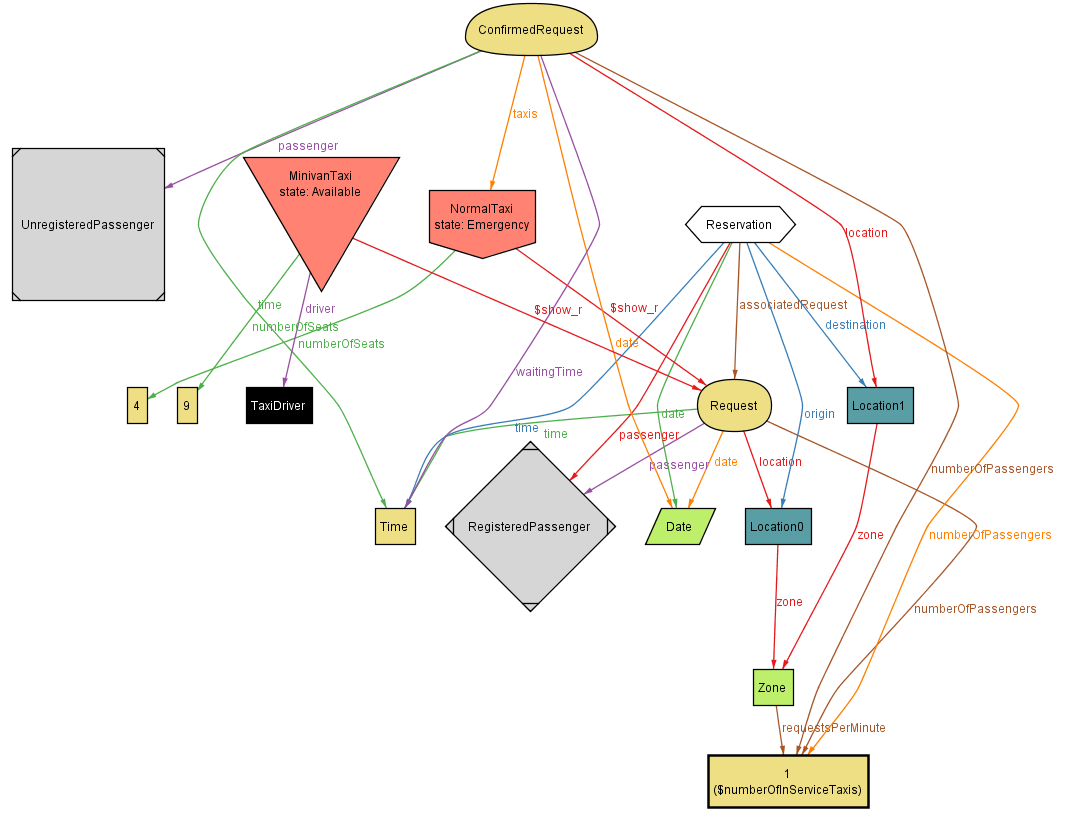
\includegraphics[scale=0.5]{alloy/instances/world1}
\par\end{centering}

\protect\caption{World generated by predicate \lstinline!pred show!}


\end{figure}


\end{landscape}

\clearpage{}

\begin{landscape}

Figure 23 is a world generated by predicate \lstinline!pred sendRequest[setOfRequests,setOfRequests': set Request, request: Request]!.
Before inserting Request2 the set of requests is composed of only
ConfirmedRequest; after the insertion also Request2 is in the set.

\begin{figure}[H]
\begin{centering}
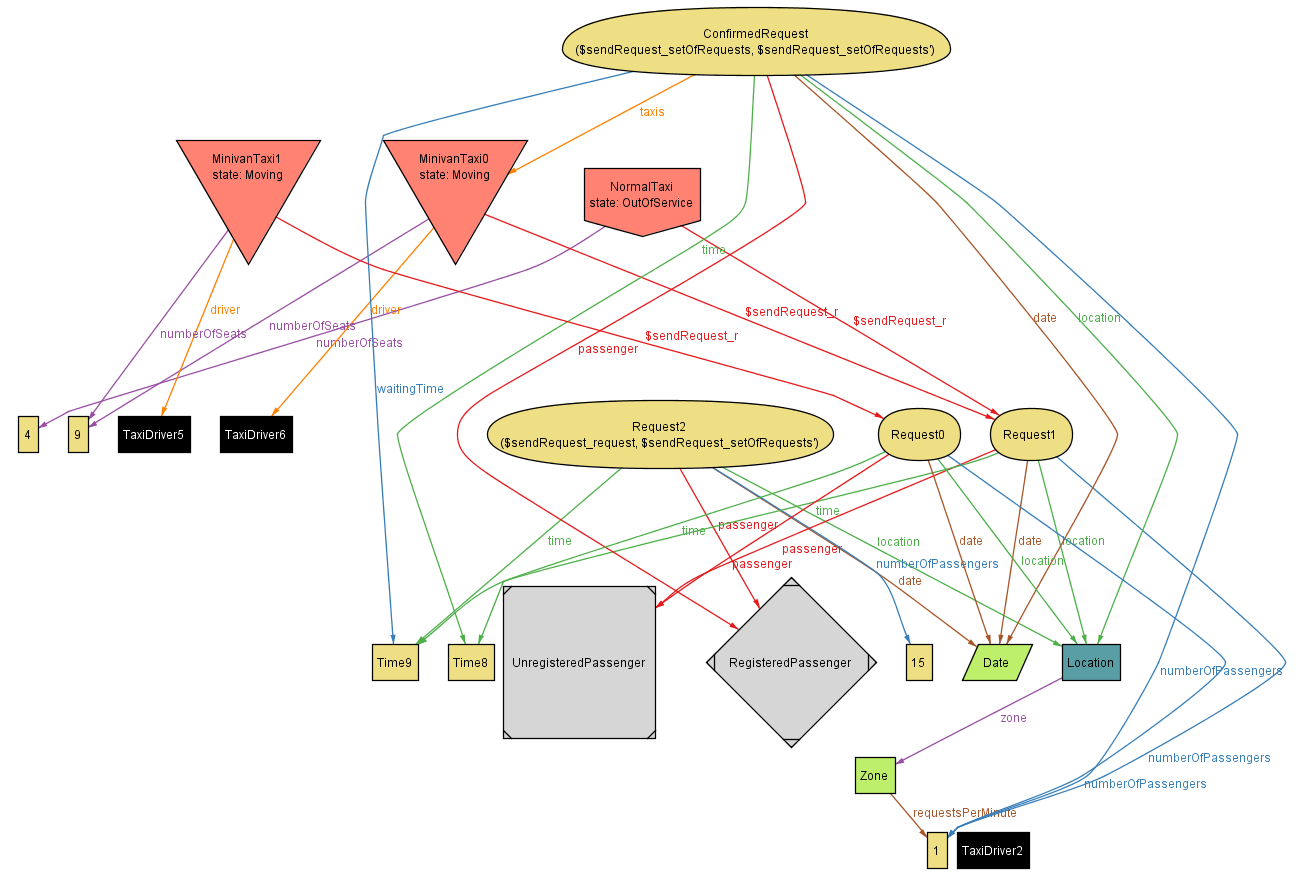
\includegraphics[scale=0.5]{alloy/instances/sendRequest}
\par\end{centering}

\protect\caption{World generated by predicate \lstinline!pred sendRequest!}
\end{figure}


\end{landscape}

\clearpage{}

\begin{landscape}

Figure 23 is a world generated by predicate \lstinline!pred sendReservation[setOfReservations,setOfReservations': set Reservation, reservation: Reservation]!.
It is clear that before the execution the set of reservation contains
only Reservation1 and after it will contain also Reservation2 (Reservation0
does not belong to any of them).

\begin{figure}[H]
\begin{centering}
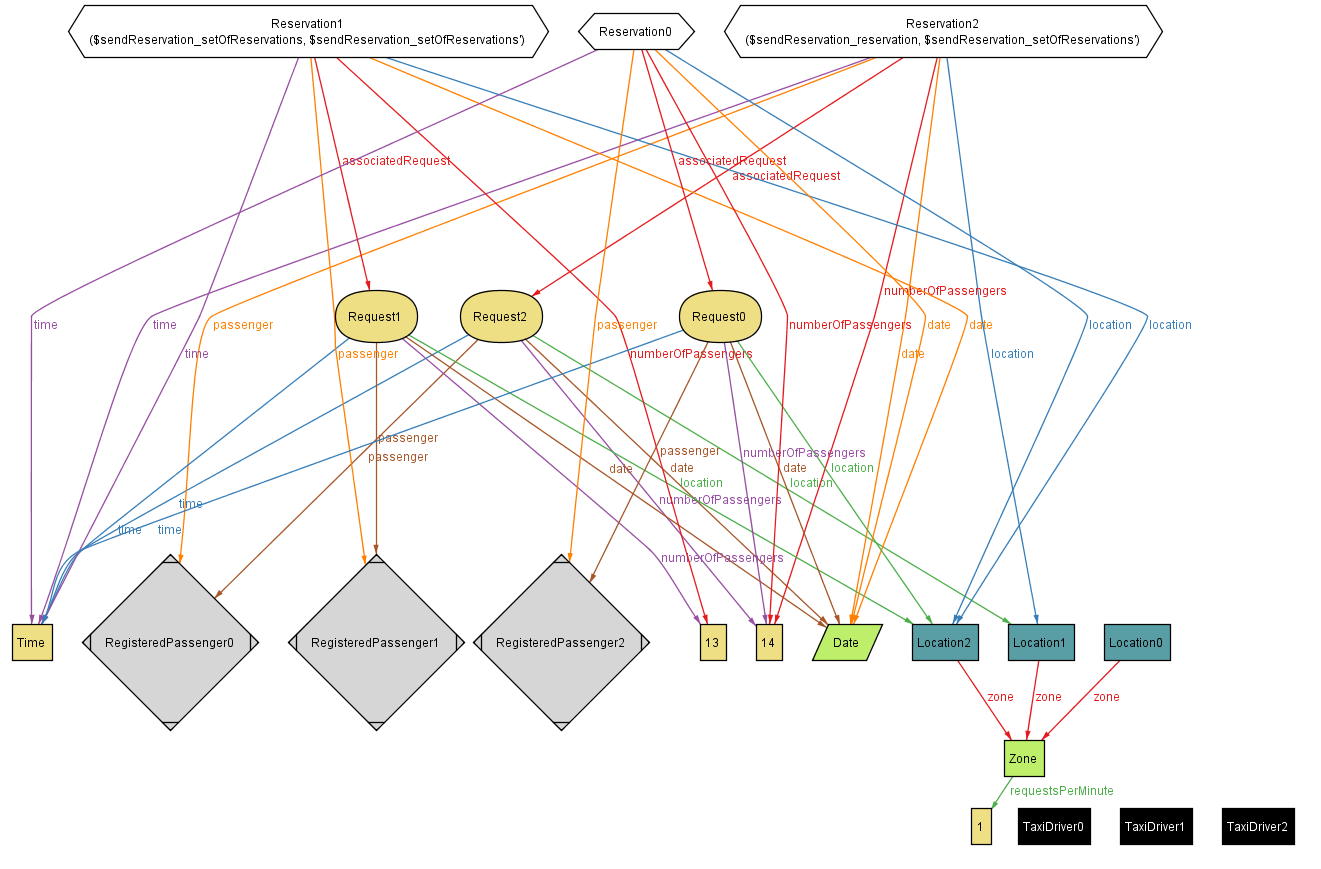
\includegraphics[scale=0.5]{alloy/instances/sendReservation}
\par\end{centering}

\protect\caption{World generated by predicate \lstinline!pred sendReservation!}
\end{figure}


\end{landscape}

\clearpage{}

\begin{landscape}

Figure 23 is a world generated by predicate \lstinline!pred cancelReservation[setOfReservations,setOfReservations': set Reservation, reservation: Reservation] !.
As you can see, before the execution Reservation1 belonged to the
set of reservation while reservation set is empty.

\begin{figure}[H]
\begin{centering}
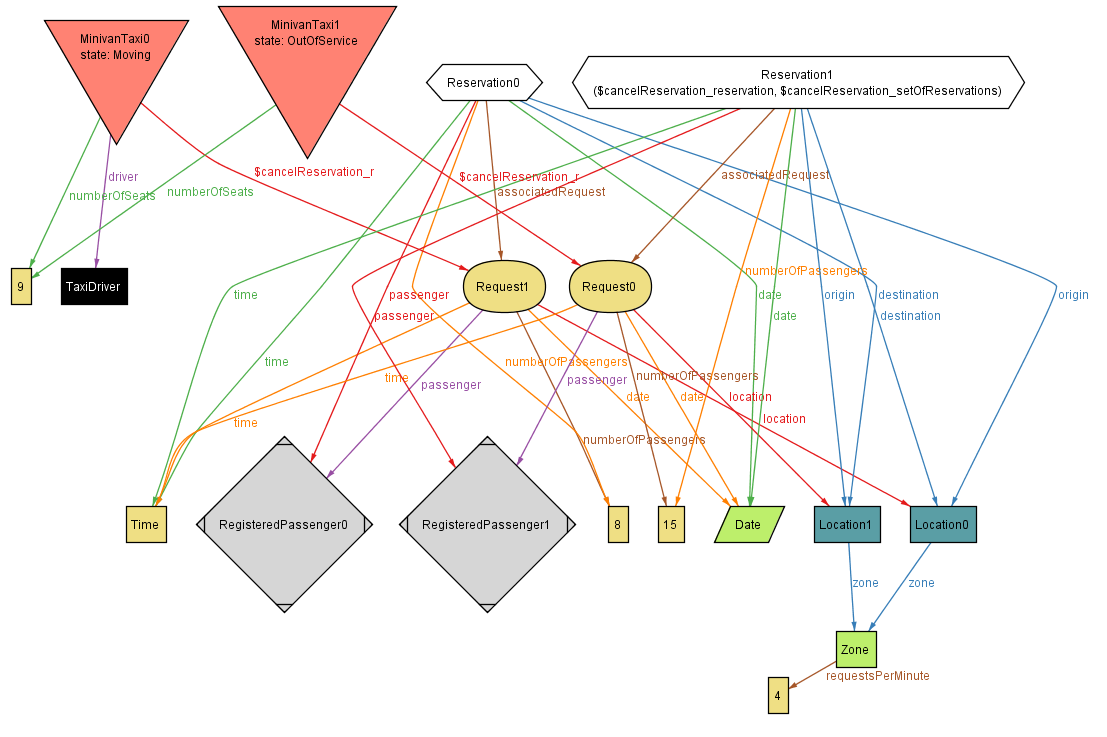
\includegraphics[scale=0.5]{alloy/instances/cancelReservation}
\par\end{centering}

\protect\caption{World generated by predicate \lstinline!pred cancelReservation!}
\end{figure}


\end{landscape}

\clearpage{}


\subsection{Queue management model}

Since queue management is a relevant part of the TS system, in this
subsection we model the structure of a queue and the adjacency relation
between zones. We will focus on the important constraints imposed
by the system but we will not model the dynamical behavior of the
queues.


\subsubsection{Signatures, facts and functions}

\begin{lstlisting}[breaklines=true]
module myTaxiService/queue

abstract sig TaxiState{} 
one sig OutOfService,Emergency extends TaxiState{} 
one sig Available, Busy, Moving extends TaxiState{}

sig Taxi { 	
	state: one TaxiState, 
}

sig Zone{ 	
	queue: one Queue, 	
	adjacentZones: some Zone, 
}

//Queue definition
sig Queue { 	
	root: lone Node 
}

sig Node { 	
	taxi: one Taxi, 	
	next: lone Node 
}

//Structural properties 
fact queueStructuralProperties { 
	
	//Each node belongs to exactly one queue 	
	all n: Node | one q: Queue | n in q.root.*next	

	//No cycles
	no n: Node | n in n.^next									 
}

//Each queue must belong to exactly one zone 
fact eachQueueBelongsToExactlyOneZone { 	
	all q: Queue | one z: Zone | q in z.queue 
}

//Adjacency relation between zones is simmetric but not reflexive 
fact adjacencySimmetricButNotReflexive 
{ 	
	adjacentZones in ~adjacentZones 	
	no adjacentZones & iden 
}

//Returns the set of taxis belonging to the queue q 
fun getTaxisFromQueue[q: Queue] : set Taxi {
	q.root.*next.taxi 
}

//Queues must store only available taxis 
fact allTaxisInQueueAreAvailable { 	
	all q: Queue | getTaxisFromQueue[q].state in Available 
}

//Each available taxi belongs to exactly one node  
	fact eachTaxiBelongsToExactlyOneNode { 	
	all t: Taxi | t.state in Available implies (one n: Node | n.taxi = t) 
} 
\end{lstlisting}



\subsubsection{Predicates}

\begin{lstlisting}
//Builds a realistic world 	
pred showQueues{ 	
	some q: Queue | #getTaxisFromQueue[q]>3 	
	some t: Taxi | t.state in OutOfService 	
	some t: Taxi | t.state in Busy 
}

run showQueues for 10 but exactly 4 Zone, exactly 10 Taxi
\end{lstlisting}


\begin{framed}
Executing "Run show for 5 but exactly 4 Zone, exactly 10 Taxi" 
Solver=sat4j Bitwidth=0 MaxSeq=0 SkolemDepth=1 Symmetry=20 
3031 vars. 176 primary vars. 6646 clauses. 15ms. 
Instance found. Predicate is consistent. 16ms.
\end{framed}


\subsubsection{Assertions}

\begin{lstlisting}[breaklines=true,showstringspaces=false]
//No available taxi are not present any queue 
assert noAvailableTaxiNotInQueue { 	
	no t: Taxi | t.state in Available and (no q:Queue | t in getTaxisFromQueue[q]) 
}

check noAvailableTaxiNotInQueue for 10
\end{lstlisting}


\begin{framed}
Executing "Check noAvailableTaxiNotInQueue for 10" 
Solver=sat4j Bitwidth=0 MaxSeq=0 SkolemDepth=1 Symmetry=20 
14039 vars. 580 primary vars. 36827 clauses. 63ms. 
No counterexample found. Assertion may be valid. 31ms.
\end{framed}

\begin{lstlisting}[breaklines=true]
//There are no taxi that appear in more than one queue
assert noTaxiSharedBetweenQueus { 	
	all disj q1,q2: Queue | no getTaxisFromQueue[q1] &  getTaxisFromQueue[q2]  
} 

check noTaxiSharedBetweenQueus for 10
\end{lstlisting}


\begin{framed}
Executing "Check noTaxiSharedBetweenQueus for 10" 
Solver=sat4j Bitwidth=0 MaxSeq=0 SkolemDepth=1 Symmetry=20 
14642 vars. 590 primary vars. 37985 clauses. 47ms. 
No counterexample found. Assertion may be valid. 531ms.
\end{framed}

\begin{figure}[H]
\begin{centering}
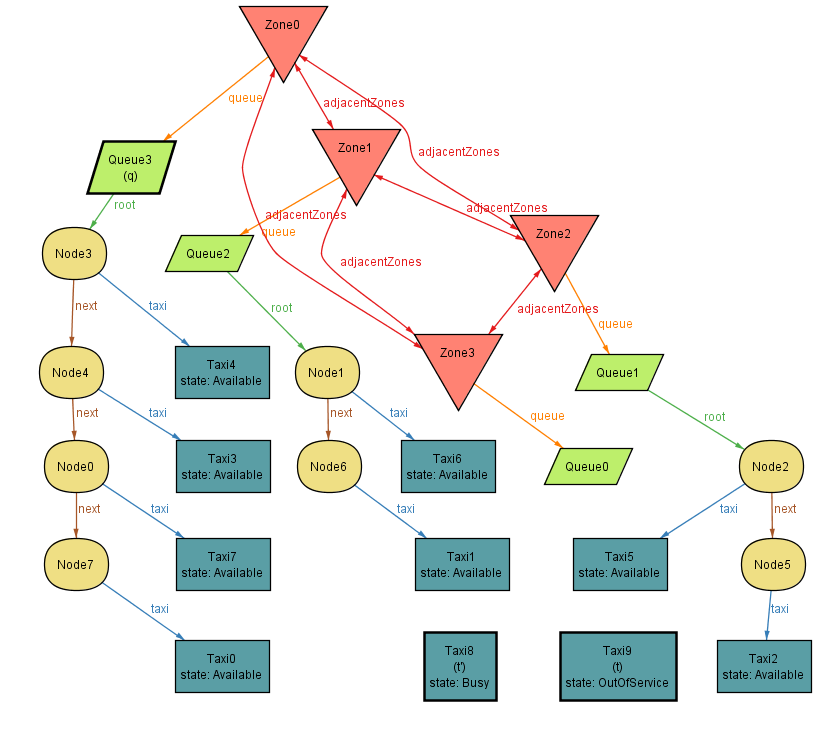
\includegraphics[scale=0.6]{alloy/instances/queues}
\par\end{centering}

\protect\caption{World generated by the predicate \lstinline!pred showQueues!}


\end{figure}



\subsection{Considerations about Alloy}

The process of modeling a complex system is always prone to many different
kinds of errors. Even though you have correctly understood the requirements
several conditions often neglected because they seem to be obvious,
but they are not. Alloy is a very precious tool that allows requirement
engineer to understand and overcome those deficiencies in the model. 


\clearpage{}

\appendix

\section{Appendix} \label{sec:Appendix1}


\subsection*{Used tools}
\begin{enumerate}
\item \LyX{} visual editor for \LaTeX{} (\url{http://www.lyx.org/}) to
write this document.
\item GanttProject for the Gantt diagram and the resource diagram \url{http://www.ganttproject.biz/}. 
\end{enumerate}

\subsection*{Hours of works}

Time spent by each group member:
\begin{itemize}
\item Alberto Maria Metelli: 10 h
\item Riccardo Mologni: 10 h
\end{itemize}

\subsection*{Revision history}
\begin{lyxlist}{00.00.0000}
\item [{%
\begin{tabular}{>{\raggedright}p{1.5cm}|>{\raggedright}p{2cm}|>{\raggedright}p{3.5cm}|>{\raggedright}p{5cm}}
\hline 
\emph{Version} & \emph{Date} & \emph{Revision description} & \emph{Revision notes}\tabularnewline
\hline 
0.1 &  & Initial draft & -\tabularnewline
\hline 
1.0 & 2-2-2016 & Final draft & -\tabularnewline
\hline 
\end{tabular}}]~\end{lyxlist}




\section*{\clearpage{}}
\end{document}
